\documentclass[notes,11pt, aspectratio=169]{beamer}

\usepackage{pgfpages}
\setbeameroption{hide notes}

\usepackage{helvet}
\usepackage[default]{lato}
\usepackage{array}
\usepackage{tgbonum}

\usepackage{tikz}
\usepackage{verbatim}
\setbeamertemplate{note page}{\pagecolor{yellow!5}\insertnote}
\usetikzlibrary{positioning}
\usetikzlibrary{calc}
\usetikzlibrary{arrows}
\usetikzlibrary{arrows.meta}
\usetikzlibrary{decorations.markings}
\usetikzlibrary{decorations.pathreplacing}
\usetikzlibrary{shapes.misc}
\usetikzlibrary{shapes.geometric}
\usetikzlibrary{matrix,shapes,arrows,fit,tikzmark}
\usepackage{amsmath}
\usepackage{amssymb}
\usepackage{mathtools}
\usepackage{bm}
\usepackage{mathpazo}
\usepackage{hyperref}
\usepackage{lipsum}
\usepackage{multimedia}
\usepackage{graphicx}
\usepackage{multirow}
\usepackage{dcolumn}
\usepackage{bbm}
\usepackage{pgfplots}
\pgfplotsset{compat=1.18}
\usepackage{listings}
\newcolumntype{d}[0]{D{.}{.}{5}}

\usepackage{changepage}
\usepackage{appendixnumberbeamer}
\newcommand{\beginbackup}{
   \newcounter{framenumbervorappendix}
   \setcounter{framenumbervorappendix}{\value{framenumber}}
   \setbeamertemplate{footline}
   {
     \leavevmode%
     \hline
     box{%
       \begin{beamercolorbox}[wd=\paperwidth,ht=2.25ex,dp=1ex,right]{footlinecolor}%
       \end{beamercolorbox}}%
     \vskip0pt%
   }
 }
\newcommand{\backupend}{
   \addtocounter{framenumbervorappendix}{-\value{framenumber}}
   \addtocounter{framenumber}{\value{framenumbervorappendix}}
}

\usepackage[space]{grffile}
\usepackage{booktabs}
\newcommand\independent{\protect\mathpalette{\protect\independenT}{\perp}}
\def\independenT#1#2{\mathrel{\rlap{$#1#2$}\mkern2mu{#1#2}}}
\DeclareMathOperator{\Supp}{Supp}
\DeclareMathOperator*{\argmin}{arg\,min}

\definecolor{blue}{RGB}{0,114,178}
\definecolor{red}{RGB}{213,94,0}
\definecolor{yellow}{RGB}{240,228,66}
\definecolor{green}{RGB}{0,158,115}

\hypersetup{
  colorlinks=true,
  linkbordercolor = {white},
  linkcolor = {blue}
}

\definecolor{MyBackground}{RGB}{255,253,218}

\newenvironment{transitionframe}{
  \setbeamercolor{background canvas}{bg=yellow}
  \begin{frame}}{
    \end{frame}
}

\setbeamercolor{frametitle}{fg=blue}
\setbeamercolor{title}{fg=black}
\setbeamertemplate{footline}[frame number]
\setbeamertemplate{navigation symbols}{}
\setbeamertemplate{itemize items}{-}
\setbeamercolor{itemize item}{fg=blue}
\setbeamercolor{itemize subitem}{fg=blue}
\setbeamercolor{enumerate item}{fg=blue}
\setbeamercolor{enumerate subitem}{fg=blue}
\setbeamercolor{button}{bg=MyBackground,fg=blue,}

\setbeamercolor{section in toc}{fg=blue}
\setbeamercolor{subsection in toc}{fg=red}
\setbeamersize{text margin left=1em,text margin right=1em}

\newenvironment{wideitemize}{\itemize\addtolength{\itemsep}{10pt}}{\enditemize}

\lstset{
    language=Python,
    basicstyle=\ttfamily\scriptsize,
    keywordstyle=\color{blue}\bfseries,
    stringstyle=\color{red!70!black},
    commentstyle=\color{green!50!black}\itshape,
    numbers=left,
    numberstyle=\tiny\color{gray},
    numbersep=5pt,
    frame=single,
    breaklines=true,
    backgroundcolor=\color{gray!5},
    showstringspaces=false,
    tabsize=4
}

\newcommand{\vx}{\mathbf{x}}
\newcommand{\vw}{\mathbf{w}}
\newcommand{\vb}{\mathbf{b}}
\newcommand{\vh}{\mathbf{h}}
\newcommand{\vy}{\mathbf{y}}
\newcommand{\vz}{\mathbf{z}}
\newcommand{\vg}{\mathbf{g}}
\newcommand{\vm}{\mathbf{m}}
\newcommand{\vv}{\mathbf{v}}
\newcommand{\vW}{\mathbf{W}}
\newcommand{\R}{\mathbb{R}}
\newcommand{\E}{\mathbb{E}}
\newcommand{\Var}{\mathrm{Var}}
\newcommand{\pd}[2]{\frac{\partial #1}{\partial #2}}


\title[]{\textcolor{blue}{Advanced Methods in Deep Learning}\\ \textcolor{black}{\normalsize Lecture 3: Training Neural Networks -- SGD, Regularization, Generalization}}
\author[Quispe]{}
\institute[MECA]{\small{Alexander Quispe Rojas \\ Universidad del Pac\'ifico -- MECA  \\ aw.quispero@up.edu.pe \quad aquisper@caltech.edu}}
\date{April 20, 2026}


\begin{document}

\tikzset{
        every picture/.style={remember picture,baseline},
        every node/.style={anchor=base,align=center,outer sep=1.5pt},
        every path/.style={thick},
        }
\tikzstyle{every picture}+=[remember picture]
\tikzstyle{mybox} =[draw=black, very thick, rectangle, inner sep=10pt, inner ysep=20pt]
\tikzstyle{fancytitle} =[draw=black,fill=red, text=white]

\begin{frame}
\maketitle
\end{frame}

\begin{frame}
\frametitle{Today's Roadmap}
\tableofcontents
\end{frame}


% ============================================================
\section{Recap and Training Challenges}
% ============================================================

\begin{transitionframe}
\begin{center}
{\Huge \textbf{Recap \& Training Challenges}}
\end{center}
\end{transitionframe}

\begin{frame}
\frametitle{Recap from Lecture 2}

\textbf{What we learned:}
\begin{wideitemize}
    \item \textbf{Backpropagation}: systematic application of the chain rule
    \[
        \bm{\delta}^{(l)} = [(\vW^{(l+1)})^\top \bm{\delta}^{(l+1)}] \odot \sigma'(\vz^{(l)})
    \]
    \item \textbf{SGD} with mini-batches:
    \[
        \vw \leftarrow \vw - \alpha \cdot \frac{1}{B}\sum_{i \in \mathcal{B}} \nabla_{\vw}\ell_i
    \]
    \item \textbf{Momentum} smooths the trajectory: $\vv_t = \beta \vv_{t-1} + \nabla\mathcal{L}$.
\end{wideitemize}

\vspace{10pt}
\textbf{Today's question:}
\begin{center}
\textcolor{red}{\Large How do we actually train deep networks \textbf{in practice}?}
\end{center}
\end{frame}

\begin{frame}
\frametitle{What Can Go Wrong During Training?}

\renewcommand{\arraystretch}{1.5}
\begin{center}
{\small
\begin{tabular}{p{4.5cm} p{5cm} p{4cm}}
\toprule
\textbf{Symptom} & \textbf{Likely cause} & \textbf{Fix (covered today)} \\
\midrule
Loss doesn't decrease & Wrong LR, bad initialization & Better optimizer, init \\
Loss oscillates wildly & LR too high, batch too small & Adaptive LR (Adam) \\
Train loss $\downarrow$ but val loss $\uparrow$ & \textcolor{red}{Overfitting} & Regularization, dropout \\
Gradients vanish/explode & Deep network, bad init & Batch norm, He init \\
Very slow convergence & Poor landscape & Momentum, Adam \\
\bottomrule
\end{tabular}
}
\end{center}

\vspace{6pt}
\textbf{Today's toolkit:} Advanced optimizers (Adam) $\cdot$ Weight initialization (Xavier, He) $\cdot$ Regularization (L1, L2, dropout) $\cdot$ Batch normalization $\cdot$ Universal Approximation Theorem $\cdot$ GPUs and parallel computing.
\end{frame}


% ============================================================
\section{Advanced Optimizers}
% ============================================================

\begin{transitionframe}
\begin{center}
{\Huge \textbf{Advanced Optimizers}}
\end{center}
\end{transitionframe}

\begin{frame}
\frametitle{The Problem with Plain SGD}

Plain SGD uses the \textbf{same learning rate} for all parameters:
\[
    \vw \leftarrow \vw - \alpha \cdot \nabla_{\vw}\mathcal{L}
\]

\vspace{4pt}
\textbf{But some parameters need different treatment:}
\begin{wideitemize}
    \item Parameters with \textbf{large} gradients: small LR needed (avoid overshooting).
    \item Parameters with \textbf{small} gradients: large LR needed (make progress).
    \item \textbf{Sparse features}: rarely updated, need larger steps when they appear.
\end{wideitemize}

\vspace{6pt}
\textbf{Solution:} \textcolor{red}{adaptive learning rates} --- each parameter gets its own step size based on its gradient history.
\end{frame}

\begin{frame}
\frametitle{AdaGrad: Adaptive Gradients}

\begin{tikzpicture}
\node [mybox] (box){%
    \begin{minipage}{0.93\textwidth}
    \vspace{-4pt}
    Accumulate squared gradients: $G_t = G_{t-1} + \vg_t \odot \vg_t$ where $\vg_t = \nabla\mathcal{L}(\vw_t)$.

    Update rule:
    \[
        \vw_{t+1} = \vw_t - \frac{\alpha}{\sqrt{G_t + \epsilon}} \odot \vg_t
    \]
    \end{minipage}
};
\node[fancytitle, right=10pt] at (box.north west) {AdaGrad (Duchi et al., 2011)};
\end{tikzpicture}

\vspace{6pt}
\textbf{Per-parameter} learning rate: $\alpha_i = \frac{\alpha}{\sqrt{G_{t,i} + \epsilon}}$.

\vspace{4pt}
\textbf{Intuition:}
\begin{itemize}
    \item Parameters with large cumulative gradients $\to$ smaller LR.
    \item Parameters with small cumulative gradients $\to$ larger LR.
\end{itemize}

\vspace{6pt}
\textcolor{red}{\textbf{Problem:}} $G_t$ grows monotonically $\Rightarrow$ LR decays to zero $\Rightarrow$ training stalls.
\end{frame}

\begin{frame}
\frametitle{RMSprop: Exponential Moving Average}

\textbf{Fix for AdaGrad:} use an \textbf{exponential moving average} instead of cumulative sum:

\begin{tikzpicture}
\node [mybox] (box){%
    \begin{minipage}{0.93\textwidth}
    \vspace{-4pt}
    \[
        \vv_t = \rho \vv_{t-1} + (1 - \rho) \vg_t \odot \vg_t
    \]
    \[
        \vw_{t+1} = \vw_t - \frac{\alpha}{\sqrt{\vv_t + \epsilon}} \odot \vg_t
    \]
    where $\rho \approx 0.9$ (typical).
    \end{minipage}
};
\node[fancytitle, right=10pt] at (box.north west) {RMSprop (Hinton, 2012)};
\end{tikzpicture}

\vspace{6pt}
\textbf{Key insight:} $\vv_t$ is a weighted average that \textbf{forgets} old gradients, so the LR doesn't decay to zero.

\vspace{6pt}
\textbf{Problem solved:} AdaGrad's aggressive LR decay. But still missing momentum.
\end{frame}

\begin{frame}
\frametitle{Adam: Momentum + RMSprop}

\textbf{Adam} combines momentum and RMSprop --- the current standard optimizer.

\vspace{4pt}
\textbf{Moment estimates:}
\begin{align*}
    \vm_t &= \beta_1 \vm_{t-1} + (1-\beta_1)\vg_t && \text{\scriptsize(first moment, like momentum)} \\
    \vv_t &= \beta_2 \vv_{t-1} + (1-\beta_2)\vg_t \odot \vg_t && \text{\scriptsize(second moment, like RMSprop)}
\end{align*}

\textbf{Bias-corrected:} \quad $\hat{\vm}_t = \dfrac{\vm_t}{1 - \beta_1^t}$ \qquad $\hat{\vv}_t = \dfrac{\vv_t}{1 - \beta_2^t}$

\vspace{4pt}
\textbf{Update:} \quad $\vw_{t+1} = \vw_t - \dfrac{\alpha \, \hat{\vm}_t}{\sqrt{\hat{\vv}_t} + \epsilon}$

\vspace{6pt}
\textbf{Defaults:} $\alpha = 10^{-3}$, $\beta_1 = 0.9$, $\beta_2 = 0.999$, $\epsilon = 10^{-8}$.
\end{frame}

\begin{frame}
\frametitle{Why Adam Works So Well}

\textbf{Adam combines three ideas:}
\begin{wideitemize}
    \item \textbf{Momentum} ($\vm_t$): smooth the gradient direction, help with noise.
    \item \textbf{Adaptive LR} ($\vv_t$): each parameter gets its own step size.
    \item \textbf{Bias correction}: crucial for the first few iterations.
\end{wideitemize}

\vspace{8pt}
\textbf{Why bias correction?} At $t = 1$, if $\vm_0 = \mathbf{0}$:
\[
    \vm_1 = (1 - \beta_1) \vg_1 \approx 0.1 \, \vg_1
\]

So $\vm_1$ is \textbf{biased toward zero}. Dividing by $1 - \beta_1^t$ corrects this:
\[
    \hat{\vm}_1 = \frac{(1 - \beta_1)\vg_1}{1 - \beta_1} = \vg_1
\]

\vspace{4pt}
\textbf{Practical advice:}
\begin{itemize}
    \item Start with \textbf{Adam}, LR = $10^{-3}$.
    \item Switch to \textbf{SGD + momentum} for final fine-tuning if needed.
\end{itemize}
\end{frame}

\begin{frame}
\frametitle{Optimizer Comparison}

\renewcommand{\arraystretch}{1.3}
\begin{center}
{\small
\begin{tabular}{lp{4.5cm}lc}
\toprule
\textbf{Optimizer} & \textbf{Update rule (schematic)} & \textbf{Hyperparams} & \textbf{Use case} \\
\midrule
SGD & $\vw \leftarrow \vw - \alpha \vg$ & $\alpha$ & Final fine-tune \\
SGD + momentum & $\vv \leftarrow \beta\vv + \vg$; $\vw \leftarrow \vw - \alpha\vv$ & $\alpha, \beta$ & Computer vision \\
AdaGrad & Cumulative $\vg^2$ scaling & $\alpha$ & Sparse / NLP \\
RMSprop & EMA of $\vg^2$ & $\alpha, \rho$ & RNNs \\
\textcolor{red}{Adam} & Momentum + RMSprop + bias corr. & $\alpha, \beta_1, \beta_2$ & \textcolor{red}{Default} \\
AdamW & Adam + decoupled weight decay & $\alpha, \beta_1, \beta_2, \lambda$ & Transformers \\
\bottomrule
\end{tabular}
}
\end{center}

\vspace{10pt}
\textbf{Rule of thumb:} When in doubt, use \textcolor{red}{Adam} with default parameters.
\end{frame}


% ============================================================
\section{Weight Initialization}
% ============================================================

\begin{transitionframe}
\begin{center}
{\Huge \textbf{Weight Initialization}}
\end{center}
\end{transitionframe}

\begin{frame}
\frametitle{Why Initialization Matters}

\textbf{Bad initialization can kill training.} Consider a few options:

\vspace{6pt}
\textcolor{red}{\textbf{Zero init}} ($\vW = \mathbf{0}$):
\begin{itemize}
    \item All neurons in a layer compute the same thing.
    \item Gradients are identical $\Rightarrow$ symmetry never breaks.
    \item Network cannot learn anything useful.
\end{itemize}

\vspace{6pt}
\textcolor{red}{\textbf{Too small}} ($\vW \sim \mathcal{N}(0, 0.01^2)$):
\begin{itemize}
    \item Activations and gradients shrink through layers.
    \item \textbf{Vanishing gradient} problem.
\end{itemize}

\vspace{6pt}
\textcolor{red}{\textbf{Too large}} ($\vW \sim \mathcal{N}(0, 1^2)$ for large layers):
\begin{itemize}
    \item Activations grow through layers.
    \item \textbf{Exploding gradient} problem.
\end{itemize}

\vspace{6pt}
\textcolor{green}{\textbf{Goal:}} Keep variance of activations roughly constant across layers.
\end{frame}

\begin{frame}
\frametitle{Xavier / Glorot Initialization}

Consider a linear layer: $z = \sum_{i=1}^{n_{in}} W_i x_i$ with $\E[x_i] = 0$, $\Var(x_i) = \sigma_x^2$.

\vspace{2pt}
Assuming $W_i$ independent with $\E[W_i] = 0$, $\Var(W_i) = \sigma_W^2$:
\[
    \Var(z) = \sum_{i=1}^{n_{in}} \Var(W_i x_i) = n_{in} \cdot \sigma_W^2 \cdot \sigma_x^2
\]

\textbf{To preserve variance} ($\Var(z) = \Var(x)$): \quad $\sigma_W^2 = \dfrac{1}{n_{in}}$

\vspace{4pt}
\begin{tikzpicture}
\node [mybox] (box){%
    \begin{minipage}{0.93\textwidth}
    \vspace{-6pt}
    \[
        W \sim \mathcal{N}\!\left(0, \frac{2}{n_{in} + n_{out}}\right)
    \]
    \vspace{-8pt}
    Designed for \textbf{tanh} / \textbf{sigmoid} activations. Uses average of $n_{in}, n_{out}$ for balance.
    \end{minipage}
};
\node[fancytitle, right=10pt] at (box.north west) {Xavier/Glorot (2010)};
\end{tikzpicture}
\end{frame}

\begin{frame}
\frametitle{He Initialization (for ReLU)}

\textbf{Problem with Xavier + ReLU:} ReLU zeroes out half the neurons, so variance halves at each layer.

\vspace{4pt}
\textbf{Fix:} double the variance to compensate.

\vspace{4pt}
\begin{tikzpicture}
\node [mybox] (box){%
    \begin{minipage}{0.93\textwidth}
    \vspace{-6pt}
    \[
        W \sim \mathcal{N}\!\left(0, \frac{2}{n_{in}}\right)
    \]
    \vspace{-8pt}
    Designed for \textbf{ReLU} activations. Used in ResNet, most modern CNNs.
    \end{minipage}
};
\node[fancytitle, right=10pt] at (box.north west) {He Initialization (2015)};
\end{tikzpicture}

\vspace{4pt}
\begin{center}
\renewcommand{\arraystretch}{1.3}
{\small
\begin{tabular}{lll}
\toprule
\textbf{Activation} & \textbf{Initialization} & \textbf{Variance} \\
\midrule
Sigmoid / Tanh & Xavier / Glorot & $2 / (n_{in} + n_{out})$ \\
ReLU / Leaky ReLU & He / Kaiming & $2 / n_{in}$ \\
\bottomrule
\end{tabular}
}
\end{center}

\vspace{2pt}
\textbf{Good news:} PyTorch uses sensible defaults; set explicitly for custom architectures.
\end{frame}


% ============================================================
\section{Regularization Techniques}
% ============================================================

\begin{transitionframe}
\begin{center}
{\Huge \textbf{Regularization}}
\end{center}
\end{transitionframe}

\begin{frame}
\frametitle{Why Regularize?}

\textbf{Deep networks can easily overfit:} millions of parameters, finite training data.

\vspace{6pt}
\textbf{Bias-variance tradeoff:}
\begin{center}
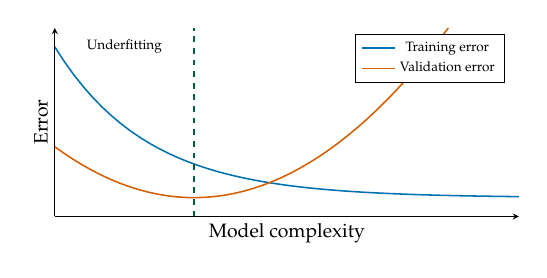
\begin{tikzpicture}[scale=0.7]
    \begin{axis}[
        xlabel={Model complexity}, ylabel={Error},
        xmin=0, xmax=10, ymin=0, ymax=5,
        width=10cm, height=5cm,
        axis lines=left, ticks=none,
        legend pos=north east,
        legend style={font=\scriptsize}
    ]
    \addplot[thick, blue, domain=0:10, samples=50] {4*exp(-0.5*x) + 0.5};
    \addlegendentry{Training error}
    \addplot[thick, red, domain=0:10, samples=50] {0.5 + 0.15*(x-3)^2};
    \addlegendentry{Validation error}
    \draw[dashed, green!60!black, thick] (axis cs:3, 0) -- (axis cs:3, 5);
    \node[green!60!black, font=\scriptsize, above] at (axis cs:3, 5) {optimal};
    \node[font=\scriptsize] at (axis cs:1.5, 4.5) {Underfitting};
    \node[font=\scriptsize] at (axis cs:8, 4.5) {Overfitting};
    \end{axis}
\end{tikzpicture}
\end{center}

\vspace{-4pt}
\textbf{Regularization:} techniques that reduce overfitting by \textbf{constraining} the model.

\vspace{4pt}
\textbf{Today we cover:} L2, L1, dropout, early stopping, data augmentation.
\end{frame}

\begin{frame}
\frametitle{L2 Regularization (Weight Decay)}

Add a penalty for large weights to the loss:

\begin{tikzpicture}
\node [mybox] (box){%
    \begin{minipage}{0.93\textwidth}
    \vspace{-4pt}
    \[
        \tilde{\mathcal{L}}(\vw) = \mathcal{L}(\vw) + \frac{\lambda}{2} \|\vw\|_2^2 = \mathcal{L}(\vw) + \frac{\lambda}{2} \sum_i w_i^2
    \]
    where $\lambda > 0$ is the regularization strength.
    \end{minipage}
};
\node[fancytitle, right=10pt] at (box.north west) {L2 Regularization};
\end{tikzpicture}

\vspace{6pt}
\textbf{Gradient:} $\nabla_{\vw} \tilde{\mathcal{L}} = \nabla_{\vw}\mathcal{L} + \lambda \vw$.

\textbf{Update rule:}
\[
    \vw \leftarrow \vw - \alpha (\nabla_{\vw}\mathcal{L} + \lambda \vw) = (1 - \alpha\lambda) \vw - \alpha \nabla_{\vw}\mathcal{L}
\]

\textcolor{red}{This is why L2 is called ``weight decay'':} weights shrink by a factor $(1 - \alpha\lambda)$ each step.

\vspace{4pt}
\textbf{Bayesian interpretation:} L2 corresponds to a \textbf{Gaussian prior} $\vw \sim \mathcal{N}(0, 1/\lambda)$ on the weights.
\end{frame}

\begin{frame}
\frametitle{L1 Regularization (Sparsity)}

\begin{tikzpicture}
\node [mybox] (box){%
    \begin{minipage}{0.93\textwidth}
    \vspace{-4pt}
    \[
        \tilde{\mathcal{L}}(\vw) = \mathcal{L}(\vw) + \lambda \|\vw\|_1 = \mathcal{L}(\vw) + \lambda \sum_i |w_i|
    \]
    \end{minipage}
};
\node[fancytitle, right=10pt] at (box.north west) {L1 Regularization};
\end{tikzpicture}

\vspace{4pt}
\textbf{Key property:} L1 induces \textbf{sparsity} --- many weights become exactly zero.

\vspace{2pt}
\begin{columns}[T]
\begin{column}{0.55\textwidth}
\textbf{Why sparsity?}

Geometric intuition: L1 constraint $|w_1| + |w_2| \leq c$ is a \textbf{diamond}. The optimum typically lies at a \textbf{corner} (axis), where some $w_i = 0$.

\vspace{6pt}
\textbf{Bayesian interpretation:} L1 = \textbf{Laplace prior} on the weights.
\end{column}

\begin{column}{0.42\textwidth}
\begin{center}
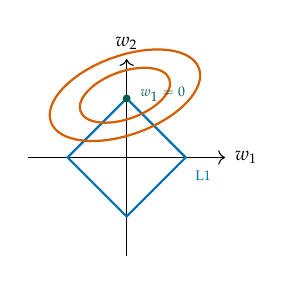
\begin{tikzpicture}[scale=0.5]
    \draw[->] (-2.5,0) -- (2.5,0) node[right, font=\scriptsize] {$w_1$};
    \draw[->] (0,-2.5) -- (0,2.5) node[above, font=\scriptsize] {$w_2$};
    \draw[thick, blue] (1.5,0) -- (0,1.5) -- (-1.5,0) -- (0,-1.5) -- cycle;
    \node[blue, font=\tiny, below right] at (1.5, -0.1) {L1};
    \draw[thick, red, rotate=20] (0.5, 1.5) ellipse (2 and 1);
    \draw[thick, red, rotate=20] (0.5, 1.5) ellipse (1.2 and 0.6);
    \fill[green!60!black] (0, 1.5) circle (0.1);
    \node[green!60!black, font=\tiny, right] at (0.1, 1.6) {$w_1 = 0$};
\end{tikzpicture}
\end{center}
\end{column}
\end{columns}
\end{frame}

\begin{frame}
\frametitle{Dropout}

\begin{tikzpicture}
\node [mybox] (box){%
    \begin{minipage}{0.93\textwidth}
    \vspace{-4pt}
    During training, randomly set a fraction $p$ of neurons to zero at each forward pass:
    \[
        \vh_{\text{drop}} = \vh \odot \vm, \qquad m_i \sim \text{Bernoulli}(1-p) \text{ independently}
    \]
    \end{minipage}
};
\node[fancytitle, right=10pt] at (box.north west) {Dropout (Srivastava et al., 2014)};
\end{tikzpicture}

\vspace{6pt}
\textbf{At inference time:} use all neurons, but \textbf{scale} by $(1-p)$ to match expected output during training.

\vspace{6pt}
\textbf{Why dropout works:}
\begin{wideitemize}
    \item \textbf{Prevents co-adaptation}: neurons can't rely on specific others.
    \item \textbf{Ensemble interpretation}: each forward pass uses a different sub-network.
    \item \textbf{Implicit regularization}: similar effect to L2.
\end{wideitemize}

\vspace{6pt}
\textbf{Typical values:} $p = 0.2$ for input layer, $p = 0.5$ for hidden layers.
\end{frame}

\begin{frame}
\frametitle{Dropout: Visual Illustration}

\begin{center}
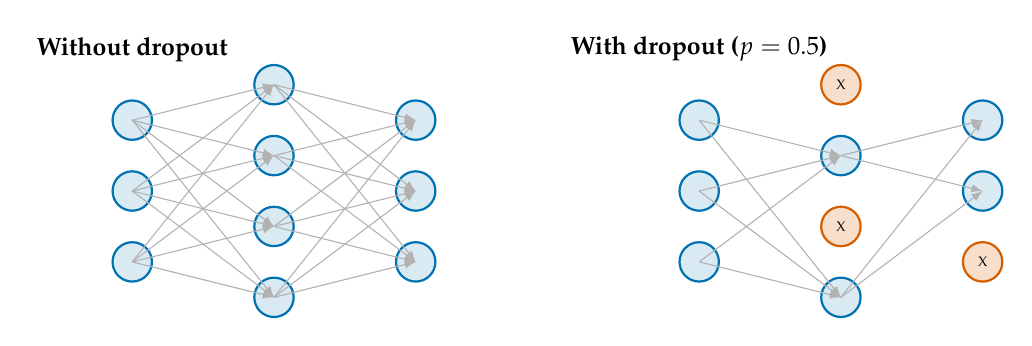
\begin{tikzpicture}[
    neuron/.style={circle, draw, thick, minimum size=0.5cm, font=\tiny},
    >=latex, scale=0.9
]
    % --- Without dropout ---
    \node[font=\small\bfseries] at (0, 3.5) {Without dropout};
    \foreach \y in {0.5, 1.5, 2.5} {
        \node[neuron, draw=blue, fill=blue!15] at (0, \y) {};
    }
    \foreach \y in {0, 1, 2, 3} {
        \node[neuron, draw=blue, fill=blue!15] at (2, \y) {};
    }
    \foreach \y in {0.5, 1.5, 2.5} {
        \node[neuron, draw=blue, fill=blue!15] at (4, \y) {};
    }
    \foreach \yi in {0.5, 1.5, 2.5} {
        \foreach \yj in {0, 1, 2, 3} {
            \draw[->, thin, gray!60] (0, \yi) -- (2, \yj);
        }
    }
    \foreach \yi in {0, 1, 2, 3} {
        \foreach \yj in {0.5, 1.5, 2.5} {
            \draw[->, thin, gray!60] (2, \yi) -- (4, \yj);
        }
    }

    % --- With dropout ---
    \node[font=\small\bfseries] at (8, 3.5) {With dropout ($p=0.5$)};
    \foreach \y in {0.5, 1.5, 2.5} {
        \node[neuron, draw=blue, fill=blue!15] at (8, \y) {};
    }
    \node[neuron, draw=blue, fill=blue!15] at (10, 0) {};
    \node[neuron, draw=red, fill=red!20] at (10, 1) {X};
    \node[neuron, draw=blue, fill=blue!15] at (10, 2) {};
    \node[neuron, draw=red, fill=red!20] at (10, 3) {X};
    \node[neuron, draw=red, fill=red!20] at (12, 0.5) {X};
    \node[neuron, draw=blue, fill=blue!15] at (12, 1.5) {};
    \node[neuron, draw=blue, fill=blue!15] at (12, 2.5) {};

    \foreach \yi in {0.5, 1.5, 2.5} {
        \foreach \yj in {0, 2} {
            \draw[->, thin, gray!60] (8, \yi) -- (10, \yj);
        }
    }
    \foreach \yi in {0, 2} {
        \foreach \yj in {1.5, 2.5} {
            \draw[->, thin, gray!60] (10, \yi) -- (12, \yj);
        }
    }
\end{tikzpicture}
\end{center}

\vspace{8pt}
\textbf{At each training step}, a different random subset of neurons is active.
\end{frame}

\begin{frame}
\frametitle{Early Stopping and Data Augmentation}

\textbf{Early stopping:} monitor validation loss and stop when it stops improving.

\begin{center}
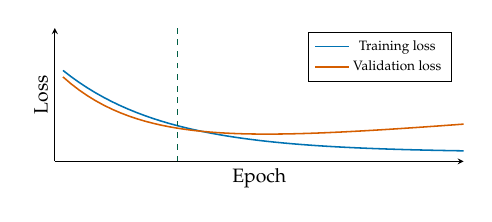
\begin{tikzpicture}[scale=0.7]
    \begin{axis}[
        xlabel={Epoch}, ylabel={Loss},
        xmin=0, xmax=50, ymin=0, ymax=3,
        width=9cm, height=4cm,
        axis lines=left, ticks=none,
        legend pos=north east,
        legend style={font=\scriptsize}
    ]
    \addplot[thick, blue, domain=1:50, samples=50] {2*exp(-0.08*x) + 0.2};
    \addlegendentry{Training loss}
    \addplot[thick, red, domain=1:50, samples=50] {2*exp(-0.1*x) + 0.3 + 0.015*(x - 15)};
    \addlegendentry{Validation loss}
    \draw[dashed, green!60!black, thick] (axis cs:15, 0) -- (axis cs:15, 3);
    \node[green!60!black, font=\scriptsize, above] at (axis cs:15, 3) {stop here};
    \end{axis}
\end{tikzpicture}
\end{center}

\vspace{-4pt}
\textbf{Data augmentation:} create ``new'' training data via transformations.
\begin{itemize}
    \item \textbf{Images:} rotation, flipping, cropping, color jittering.
    \item \textbf{Text:} synonym replacement, back-translation.
    \item \textbf{Time series:} jittering, time warping.
    \item \textbf{Effect:} teach the model \textbf{invariances}.
\end{itemize}
\end{frame}


% ============================================================
\section{Batch Normalization}
% ============================================================

\begin{transitionframe}
\begin{center}
{\Huge \textbf{Batch Normalization}}
\end{center}
\end{transitionframe}

\begin{frame}
\frametitle{The Internal Covariate Shift Problem}

In a deep network, the distribution of activations at each layer \textbf{changes} during training (as earlier layers' weights change).

\vspace{6pt}
\textbf{Consequences:}
\begin{wideitemize}
    \item Each layer must constantly adapt to its input distribution.
    \item Training is slower.
    \item Requires careful initialization and small learning rates.
\end{wideitemize}

\vspace{8pt}
\textbf{Idea (Ioffe \& Szegedy, 2015):} \textcolor{red}{normalize activations} at each layer to have mean 0 and variance 1.

\vspace{6pt}
\textbf{But naive normalization destroys information.} The solution: normalize, then learn scale and shift.
\end{frame}

\begin{frame}
\frametitle{Batch Normalization: The Algorithm}

For a mini-batch $\mathcal{B} = \{x_1, \ldots, x_B\}$:

\vspace{4pt}
\textbf{Step 1 -- Compute batch statistics:}
\[
    \mu_{\mathcal{B}} = \frac{1}{B}\sum_{i=1}^{B} x_i \qquad \sigma_{\mathcal{B}}^2 = \frac{1}{B}\sum_{i=1}^{B} (x_i - \mu_{\mathcal{B}})^2
\]

\textbf{Step 2 -- Normalize:} \quad $\hat{x}_i = \dfrac{x_i - \mu_{\mathcal{B}}}{\sqrt{\sigma_{\mathcal{B}}^2 + \epsilon}}$

\vspace{6pt}
\textbf{Step 3 -- Scale and shift (learnable):} \quad $y_i = \gamma \hat{x}_i + \beta$

\vspace{4pt}
where $\gamma, \beta$ are \textbf{learned parameters} (via backprop).

\vspace{6pt}
\textcolor{red}{\textbf{Key insight:}} if the network learns $\gamma = \sigma_{\mathcal{B}}, \beta = \mu_{\mathcal{B}}$, BN is identity $\Rightarrow$ no loss of expressiveness.
\end{frame}

\begin{frame}
\frametitle{Batch Norm: Training vs Inference}

\textbf{At training time:} use \textbf{batch statistics} $\mu_{\mathcal{B}}, \sigma_{\mathcal{B}}^2$.

\vspace{6pt}
\textbf{At inference time:} batches may have size 1, so batch statistics are unreliable.

\textbf{Solution:} maintain \textbf{running averages} during training:
\begin{align*}
    \mu_{\text{run}} &\leftarrow (1 - m)\mu_{\text{run}} + m \mu_{\mathcal{B}} \\
    \sigma_{\text{run}}^2 &\leftarrow (1 - m)\sigma_{\text{run}}^2 + m \sigma_{\mathcal{B}}^2
\end{align*}

At inference, use $\mu_{\text{run}}, \sigma_{\text{run}}^2$.

\vspace{6pt}
\textbf{Benefits of BN:}
\begin{itemize}
    \item \textcolor{green}{Faster training} (allows higher LR).
    \item \textcolor{green}{Smoother loss landscape} (shown empirically).
    \item \textcolor{green}{Implicit regularization} (batch noise acts as regularization).
    \item \textcolor{green}{Less sensitive to initialization}.
\end{itemize}

\vspace{4pt}
\textbf{Variants:} Layer Norm (Transformers), Group Norm, Instance Norm.
\end{frame}


% ============================================================
\section{Universal Approximation Theorem}
% ============================================================

\begin{transitionframe}
\begin{center}
{\Huge \textbf{Universal Approximation Theorem}}
\end{center}
\end{transitionframe}

\begin{frame}
\frametitle{The Universal Approximation Theorem}

\begin{tikzpicture}
\node [mybox] (box){%
    \begin{minipage}{0.93\textwidth}
    \vspace{-4pt}
    Let $\sigma$ be a non-constant, bounded, monotonically increasing continuous function. Then for any continuous function $f: [0,1]^d \to \R$ and any $\epsilon > 0$, there exist $N \in \mathbb{N}$, $\{w_i\}, \{b_i\}, \{v_i\}$ such that:
    \[
        \left| f(\vx) - \sum_{i=1}^{N} v_i \, \sigma(\vw_i^\top \vx + b_i) \right| < \epsilon \quad \forall \vx \in [0,1]^d
    \]

    \textbf{In words:} a neural network with \textbf{one hidden layer} and \textbf{enough neurons} can approximate any continuous function to arbitrary precision.
    \end{minipage}
};
\node[fancytitle, right=10pt] at (box.north west) {Cybenko (1989), Hornik (1991)};
\end{tikzpicture}

\vspace{6pt}
\textbf{Extensions:}
\begin{itemize}
    \item Works for sigmoid, tanh, ReLU (with adjustments).
    \item Also holds for any Lebesgue-measurable function.
\end{itemize}
\end{frame}

\begin{frame}
\frametitle{UAT: Proof Sketch (Geometric Intuition)}

\textbf{Goal:} approximate any function $f(x)$ with a sum of sigmoids.

\vspace{4pt}
\textbf{Step 1:} A single sigmoid can approximate a \textbf{step function} (with large $w$):
\[
    \sigma(wx + b) \approx \begin{cases} 1 & x > -b/w \\ 0 & x < -b/w \end{cases} \quad \text{for large } w
\]

\textbf{Step 2:} Two sigmoids with opposite weights create a \textbf{bump} function:
\[
    \sigma(w(x - a)) - \sigma(w(x - a - h)) \approx \text{bump on } [a, a+h]
\]

\textbf{Step 3:} Sum many bumps $\to$ approximate any continuous function (like Riemann integration!).

\vspace{8pt}
\textbf{Formal argument:} uses the Hahn-Banach theorem + Riesz representation theorem.

\vspace{6pt}
\begin{center}
\textcolor{red}{\textbf{Key insight:} sigmoids form a dense subset of continuous functions on compact sets.}
\end{center}
\end{frame}

\begin{frame}
\frametitle{But Why Depth Then?}

\textbf{UAT says:} one hidden layer is enough. But in practice, we use \textbf{deep} networks.

\vspace{6pt}
\textbf{Problem with shallow networks:} the required width can grow \textbf{exponentially} with complexity.

\vspace{6pt}
\begin{tikzpicture}
\node [mybox] (box){%
    \begin{minipage}{0.93\textwidth}
    \vspace{-4pt}
    \textbf{Depth-width tradeoff (Telgarsky, 2016):}

    There exist functions that can be represented by a network of depth $L$ with $O(L)$ neurons, but require $\Omega(2^L)$ neurons in a shallow network.
    \end{minipage}
};
\node[fancytitle, right=10pt] at (box.north west) {Theorem};
\end{tikzpicture}

\vspace{8pt}
\textbf{Why deep works:}
\begin{wideitemize}
    \item \textbf{Hierarchical features}: edges $\to$ parts $\to$ objects.
    \item \textbf{Compositional structure}: natural data is compositional.
    \item \textbf{Exponential efficiency}: depth is \textbf{exponentially more parameter-efficient}.
\end{wideitemize}
\end{frame}

\begin{frame}
\frametitle{Why Depth Matters -- Economic Analogy}

\textbf{Deep networks learn hierarchical representations:}

\vspace{6pt}
\begin{center}
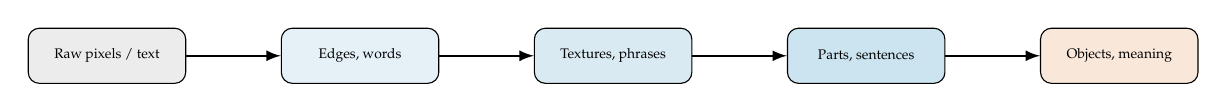
\begin{tikzpicture}[
    node distance=0.3cm and 1.2cm,
    box/.style={rectangle, draw, rounded corners, minimum height=0.7cm, minimum width=2cm, align=center, font=\tiny},
    >=latex
]
    \node[box, fill=gray!15] (input) {Raw pixels / text};
    \node[box, fill=blue!10, right=of input] (l1) {Edges, words};
    \node[box, fill=blue!15, right=of l1] (l2) {Textures, phrases};
    \node[box, fill=blue!20, right=of l2] (l3) {Parts, sentences};
    \node[box, fill=red!15, right=of l3] (out) {Objects, meaning};

    \draw[->, thick] (input) -- (l1);
    \draw[->, thick] (l1) -- (l2);
    \draw[->, thick] (l2) -- (l3);
    \draw[->, thick] (l3) -- (out);
\end{tikzpicture}
\end{center}

\vspace{6pt}
\textbf{Analogy with economics:}
\begin{wideitemize}
    \item Raw data: prices, quantities, transactions.
    \item Layer 1: growth rates, ratios, simple features.
    \item Layer 2: trends, seasonality, co-movements.
    \item Layer 3: regime indicators, crisis flags.
    \item Output: GDP forecast, policy recommendation.
\end{wideitemize}

\vspace{4pt}
\textcolor{red}{Economic relationships are often compositional --- which is why depth helps.}
\end{frame}


% ============================================================
\section{GPUs and Parallel Computing}
% ============================================================

\begin{transitionframe}
\begin{center}
{\Huge \textbf{GPUs and Parallel Computing}}
\end{center}
\end{transitionframe}

\begin{frame}
\frametitle{CPU vs GPU Architecture}

\begin{columns}[T]
\begin{column}{0.48\textwidth}
\centering
\textcolor{blue}{\textbf{CPU}}

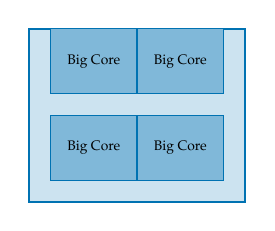
\begin{tikzpicture}[scale=0.55]
    \draw[fill=blue!20, draw=blue, thick] (0,0) rectangle (5, 4);
    \foreach \x in {0.5, 2.5} {
        \foreach \y in {0.5, 2.5} {
            \draw[fill=blue!50, draw=blue] (\x, \y) rectangle (\x+2, \y+1.5);
        }
    }
    \node[font=\tiny] at (1.5, 1.25) {Big Core};
    \node[font=\tiny] at (3.5, 1.25) {Big Core};
    \node[font=\tiny] at (1.5, 3.25) {Big Core};
    \node[font=\tiny] at (3.5, 3.25) {Big Core};
\end{tikzpicture}

\begin{itemize}
    \item Few powerful cores (4--64).
    \item Optimized for \textbf{sequential} execution.
    \item Great for branching logic.
\end{itemize}
\end{column}

\begin{column}{0.48\textwidth}
\centering
\textcolor{red}{\textbf{GPU}}

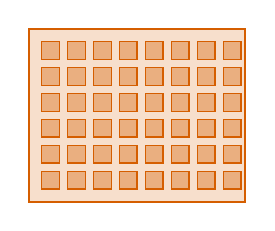
\begin{tikzpicture}[scale=0.55]
    \draw[fill=red!20, draw=red, thick] (0,0) rectangle (5, 4);
    \foreach \x in {0.3, 0.9, 1.5, 2.1, 2.7, 3.3, 3.9, 4.5} {
        \foreach \y in {0.3, 0.9, 1.5, 2.1, 2.7, 3.3} {
            \draw[fill=red!50, draw=red] (\x, \y) rectangle (\x+0.4, \y+0.4);
        }
    }
\end{tikzpicture}

\begin{itemize}
    \item Thousands of simple cores.
    \item Optimized for \textbf{parallel} execution.
    \item Great for matrix operations.
\end{itemize}
\end{column}
\end{columns}

\vspace{6pt}
\textbf{Why GPUs dominate DL:} neural networks are mostly \textbf{matrix multiplications}, which are embarrassingly parallel. A $1000 \times 1000$ matmul: CPU = seconds, GPU = milliseconds.
\end{frame}

\begin{frame}[fragile]
\frametitle{Using GPUs in PyTorch}

\begin{lstlisting}
import torch

# Check if GPU is available
device = torch.device('cuda' if torch.cuda.is_available() else 'cpu')
print(f"Using device: {device}")

# Move tensors to GPU
x = torch.randn(1000, 1000).to(device)
y = torch.randn(1000, 1000).to(device)
z = x @ y                    # Matmul on GPU

# Move model to GPU
model = MyNeuralNetwork().to(device)

# Move batches to GPU during training
for X_batch, y_batch in loader:
    X_batch, y_batch = X_batch.to(device), y_batch.to(device)
    y_pred = model(X_batch)
    loss = criterion(y_pred, y_batch)
\end{lstlisting}

\textbf{Rule:} both model and data must be on the \textbf{same device}.
\end{frame}

\begin{frame}
\frametitle{Parallelism Strategies}

\textbf{Data parallelism} (most common):
\begin{itemize}
    \item Replicate model across multiple GPUs.
    \item Split batch across GPUs.
    \item Average gradients after each step.
    \item PyTorch: \texttt{nn.DataParallel}, \texttt{nn.DistributedDataParallel}.
\end{itemize}

\vspace{6pt}
\textbf{Model parallelism} (for huge models):
\begin{itemize}
    \item Split model across multiple GPUs.
    \item Used for LLMs that don't fit in one GPU.
\end{itemize}

\vspace{6pt}
\textbf{Mixed precision training (AMP):}
\begin{itemize}
    \item Use float16 instead of float32 where possible.
    \item \textbf{2x faster} on modern GPUs (tensor cores).
    \item PyTorch: \texttt{torch.cuda.amp.autocast}.
\end{itemize}

\vspace{6pt}
\textbf{For this course:} Google Colab GPUs are enough (T4, A100).
\end{frame}


% ============================================================
\section{Practical Recipe and Summary}
% ============================================================

\begin{transitionframe}
\begin{center}
{\Huge \textbf{Practical Recipe \& Summary}}
\end{center}
\end{transitionframe}

\begin{frame}
\frametitle{The Deep Learning Training Recipe}

A checklist for training deep networks:

\begin{enumerate}
    \item \textbf{Normalize your inputs} (mean 0, std 1 per feature).
    \item \textbf{Initialize weights properly:} He (ReLU) or Xavier (sigmoid/tanh).
    \item \textbf{Choose architecture:} start simple, add complexity as needed.
    \item \textbf{Add batch normalization} to hidden layers.
    \item \textbf{Pick optimizer:} start with \textbf{Adam} (LR = $10^{-3}$).
    \item \textbf{Add regularization:} dropout (0.2-0.5) or weight decay ($10^{-4}$).
    \item \textbf{Monitor train and validation loss} at each epoch.
    \item \textbf{Use early stopping} based on validation loss.
    \item \textbf{Scale up}: batch size, depth, width, data augmentation.
\end{enumerate}

\vspace{6pt}
\textbf{Debugging tips:}
\begin{itemize}
    \item If loss is NaN: LR too high or bad init.
    \item If loss doesn't decrease: check gradients, try different optimizer.
    \item If overfitting: more regularization, more data, smaller model.
\end{itemize}
\end{frame}

\begin{frame}
\frametitle{Lecture 3 Summary}

\begin{enumerate}
    \item \textbf{Optimizers:} Adam combines momentum + adaptive LR + bias correction. Default choice.

    \item \textbf{Initialization:} Xavier for sigmoid/tanh, He for ReLU.

    \item \textbf{Regularization:} L2 shrinks weights, L1 induces sparsity, dropout breaks co-adaptation.

    \item \textbf{Batch Normalization:} normalize activations per batch, with learnable $\gamma, \beta$.

    \item \textbf{UAT:} one hidden layer is enough \textit{in theory}, but depth is \textbf{exponentially more efficient} for compositional functions.

    \item \textbf{GPUs:} parallelism enables training of large models. Use PyTorch \texttt{.to(device)}.
\end{enumerate}
\end{frame}

\begin{frame}
\frametitle{Next Lecture: Convolutional Neural Networks}

\textbf{Lecture 4} (Saturday, April 25):
\begin{itemize}
    \item Motivation: why CNNs for images?
    \item The convolution operation (mathematical details).
    \item Pooling and modern alternatives.
    \item Classic architectures: LeNet, AlexNet, VGG, ResNet.
    \item Applications: satellite imagery for poverty prediction.
\end{itemize}

\vspace{6pt}
\textbf{Recommended reading:}
\begin{itemize}
    \item Goodfellow et al., \textit{Deep Learning}, Chapters 7--8.
    \item Kingma \& Ba (2015), \textit{Adam}; Ioffe \& Szegedy (2015), \textit{Batch Normalization}.
\end{itemize}

\vspace{6pt}
\textcolor{red}{\textbf{Homework 1 is now available!}} Due Sunday, April 27. Covers Lectures 1--3.

\vspace{4pt}
\begin{center}
\Large \textcolor{blue}{\textbf{Questions?}}
\end{center}
\end{frame}

\begin{frame}
\frametitle{References}

\footnotesize
\begin{itemize}
    \item Kingma, D. P., \& Ba, J. (2015). Adam: A method for stochastic optimization. \textit{ICLR}.
    \item Duchi, J., Hazan, E., \& Singer, Y. (2011). Adaptive subgradient methods. \textit{JMLR}, 12, 2121--2159.
    \item Glorot, X., \& Bengio, Y. (2010). Understanding the difficulty of training deep feedforward neural networks. \textit{AISTATS}.
    \item He, K., Zhang, X., Ren, S., \& Sun, J. (2015). Delving deep into rectifiers. \textit{ICCV}.
    \item Srivastava, N. et al. (2014). Dropout: A simple way to prevent neural networks from overfitting. \textit{JMLR}.
    \item Ioffe, S., \& Szegedy, C. (2015). Batch normalization. \textit{ICML}.
    \item Cybenko, G. (1989). Approximation by superpositions of a sigmoidal function. \textit{Math. Control Signals Syst}.
    \item Hornik, K. (1991). Approximation capabilities of multilayer feedforward networks. \textit{Neural Networks}.
\end{itemize}
\end{frame}

\end{document}
